\subsection{原理と方法}

\paragraph{モデル}
一次元の線形状態空間モデルを用いる:
\[
  \theta_k = a_k\,\theta_{k-1} + v_k,\tag{3.40}
\]
\[
  y_k = c_k\,\theta_k + w_k,\tag{3.41}
\]
ここで $v_k\sim\mathcal N(0,\sigma_v^2)$,$w_k\sim\mathcal N(0,\sigma_w^2)$ は互いに独立で白色,$a_k,c_k$ は既知とする\cite{exp2025}。目的は「時刻 $k$ までの観測 $\{y_\ell\}_{\ell=1}^k$ に基づく $\theta_k$ の最小平均二乗誤差(MMSE)推定」を行うこと\cite{exp2025}。

以下はこのモデルに基づくデータ生成のRによる実装例である。
\begin{lstlisting}[language=R,caption={データ生成関数}]
# データ生成関数(exp11とexp12で共通使用)
generate_kalman_data <- function(seed = 123, N = 100, a_k = 0.9, c_k = 2, 
                                  sigma2_v = 1, sigma2_w = 1) {
  # 乱数シードを設定
  set.seed(seed)
  
  # 初期値
  theta_0 <- rnorm(1, mean = 3, sd = sqrt(2))  # θ_0 ~ N(3, 2)
  V_0 <- 2
  
  # データ格納用
  theta_true <- numeric(N)
  y_obs <- numeric(N)
  
  # 初期化
  theta_k_1 <- theta_0
  
  # データ生成
  for (k in 1:N) {
    # 真の状態遷移 (3.40): θ_k = a_k * θ_{k-1} + v_k
    v_k <- rnorm(1, mean = 0, sd = sqrt(sigma2_v))
    theta_k <- a_k * theta_k_1 + v_k
    theta_true[k] <- theta_k
    
    # 観測 (3.41): y_k = c_k * θ_k + w_k
    w_k <- rnorm(1, mean = 0, sd = sqrt(sigma2_w))
    y_k <- c_k * theta_k + w_k
    y_obs[k] <- y_k
    
    # 次のステップへ
    theta_k_1 <- theta_k
  }
  
  # データを返す
  return(list(
    theta_true = theta_true,
    y_obs = y_obs,
    theta_0 = theta_0,
    V_0 = V_0,
    a_k = a_k,
    c_k = c_k,
    sigma2_v = sigma2_v,
    sigma2_w = sigma2_w,
    N = N
  ))
}
\end{lstlisting}

\paragraph{Kalman フィルタ}
平方完成による最適ゲイン $F_k$ と分散更新を導くと,予測分散 $X_k$,事後分散 $V_k$,推定値 $\hat\theta_k$ は
\[
\hat\theta_k = a_k\hat\theta_{k-1} + F_k\bigl(y_k - c_k a_k \hat\theta_{k-1}\bigr),\tag{3.36}
\]
\[
X_k = a_k^2 V_{k-1} + \sigma_v^2,\tag{3.37}
\]
\[
V_k = \frac{\sigma_w^2\, X_k}{c_k^2 X_k + \sigma_w^2},\tag{3.38}
\]
\[
F_k = \frac{c_k X_k}{c_k^2 X_k + \sigma_w^2}.\tag{3.39}
\]
これが Kalman フィルタであり,推定誤差分散を最小にする\cite{exp2025}。初期条件は $\hat\theta_0=\bar\theta,\;V_0=P$ とする\cite{exp2025}。

以下は、KalmanフィルタのRによる実装例である。

\begin{lstlisting}[language=R,caption={Kalmanフィルタ更新(式(3.36)–(3.39))}]
update_kalman_filter <- function(theta_k_1, V_k_1, y_k, a_k, c_k, sigma2_v, sigma2_w) {
  # (3.37) 予測分散
  X_k <- a_k^2 * V_k_1 + sigma2_v
  # (3.39) カルマンゲイン
  F_k <- (c_k * X_k) / (c_k^2 * X_k + sigma2_w)
  # (3.36) 推定値更新
  theta_k <- a_k * theta_k_1 + F_k * (y_k - c_k * a_k * theta_k_1)
  # (3.38) 事後分散更新
  V_k <- (sigma2_w * X_k) / (c_k^2 * X_k + sigma2_w)
  list(theta_k = theta_k, V_k = V_k, X_k = X_k, F_k = F_k)
}
\end{lstlisting}

\paragraph{Kalman スムーザ}
全データ $\{y_1,\dots,y_N\}$ を用いて各 $\theta_k$ を後処理で精密化する。Rauch–Tung–Striebel(RTS)型の退行更新は
\[
\hat\theta_k^{\,s}=\hat\theta_k + g_k\bigl(\hat\theta_{k+1}^{\,s}-a_k\hat\theta_k\bigr),\tag{3.42}
\]
\[
g_k=\frac{a_k V_k}{X_{k+1}},\tag{3.43}
\]
\[
V_k^{\,s}=V_k + g_k^2\bigl(V_{k+1}^{\,s}-X_{k+1}\bigr),\tag{3.44}
\]
終端条件は $\hat\theta_N^{\,s}=\hat\theta_N,\;V_N^{\,s}=V_N$。$\{\hat\theta_k^{\,s}\}$ は時刻 $N$ までの全情報に基づく MMSE 推定となる\cite{exp2025}。

以下は、KalmanスムーザのRによる実装例である。

\begin{lstlisting}[language=R,caption={Kalmanスムーザ更新(式(3.42)–(3.44))}]
update_kalman_smoother <- function(theta_k, theta_k_plus_1_s, V_k, V_k_plus_1_s, X_k_plus_1, a_k) {
  # (3.43) 後向きゲイン
  g_k <- a_k * V_k / X_k_plus_1
  # (3.42) 推定値の後向き補正
  theta_k_s <- theta_k + g_k * (theta_k_plus_1_s - a_k * theta_k)
  # (3.44) 分散の後向き補正
  V_k_s <- V_k + g_k^2 * (V_k_plus_1_s - X_k_plus_1)
  list(theta_k_s = theta_k_s, V_k_s = V_k_s, g_k = g_k)
}
\end{lstlisting}

\subsection{課題11(カルマンフィルタ:フォワード)}
\label{subsec:task11}

\paragraph{内容}
一次元状態空間モデルを対象とする.
\begin{align}
  \theta_k &= a_k\,\theta_{k-1} + v_{k-1}, \quad v_{k-1}\sim \mathcal{N}(0,\sigma_v^2),\\
  y_k &= c_k\,\theta_k + w_k, \quad w_k\sim \mathcal{N}(0,\sigma_w^2).
\end{align}
初期推定値は$\hat{\theta}_0=\theta_0$, 分散$V_0$を与える.
評価は平均二乗誤差
\begin{align}
  \mathrm{MSE}=\frac{1}{N}\sum_{k=1}^{N}\bigl(\theta_k^{\mathrm{true}}-\hat{\theta}_k\bigr)^2
\end{align}
で行う.

\paragraph{方法}
時刻$k$ごとに予測と更新を行う.
\begin{align}
  X_k &= a_k^2 V_{k-1} + \sigma_v^2,\\
  F_k &= \frac{c_k X_k}{c_k^2 X_k + \sigma_w^2},\\
  \hat{\theta}_k &= a_k \hat{\theta}_{k-1} + F_k\bigl(y_k - c_k a_k \hat{\theta}_{k-1}\bigr),\\
  V_k &= (1 - F_k c_k)\,X_k.
\end{align}
出力は$\{\hat{\theta}_k\}_{k=1}^N$と$\{V_k\}_{k=1}^N$.

\paragraph{実装}
関数\verb|exp11(data)|を用いる.各$k$で\verb|update_kalman_filter|を呼び,$X_k, F_k, \hat{\theta}_k, V_k$を更新する.推定系列と真値を重ね描画し\verb|graphs/task11.png|に保存する.

\paragraph{結果}
データ生成と実行条件は
\begin{verbatim}
kalman_data <- generate_kalman_data(seed = 42, N = 100,
                                    a_k = 0.9, c_k = 2,
                                    sigma2_v = 1, sigma2_w = 1)
result11 <- exp11(kalman_data)
\end{verbatim}
である.MSEは\verb|mmse: 0.1935684| となった.図\ref{fig:task11_fig}に真値と推定の系列を示す.

\begin{figure}[H]
  \centering
  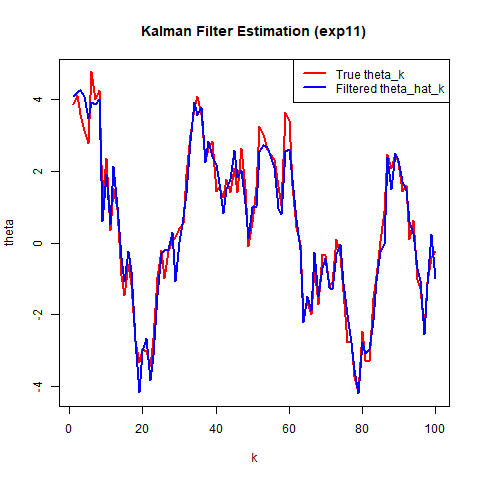
\includegraphics[width=0.8\linewidth]{graphs/task11.png}
  \caption{カルマンフィルタ(フォワード)による推定結果(赤:真値,青:推定)}
  \label{fig:task11_fig}
\end{figure}

\paragraph{考察}
% ここに記述


